\documentclass{article}%
\usepackage[T1]{fontenc}%
\usepackage[utf8]{inputenc}%
\usepackage{lmodern}%
\usepackage{textcomp}%
\usepackage{lastpage}%
\usepackage{authblk}%
\usepackage{graphicx}%
%
\title{Functional CD40 Expression Induced following Bacterial Infection of Mouse and Human Osteoblast}%
\author{Bruce Compton}%
\affil{Department of Biochemistry, Institute of Medical Sciences, Banaras Hindu University, Varanasi, India}%
\date{01{-}01{-}2013}%
%
\begin{document}%
\normalsize%
\maketitle%
\section{Abstract}%
\label{sec:Abstract}%
SAN DIEGO, Calif. {-} Two more mature tumor cells exposed to a compound called miR{-}221 could represent powerful new targets for new therapies in breast and prostate cancer, researchers reported in a new study in OncoMolecular, the journal of Oncogene, a nonprofit research nonprofit that focuses on discovering, evaluating and applying predictive biomarkers and markers to develop personalized cancer treatments.\newline%
The two new posters for OncoMolecular will be available at www.onifemolecular.org.\newline%
The findings demonstrate a very versatile and high{-}potential target in the mix of today's most promising cancer drugs, according to lead researcher Dr. Dan Gerson, chief of translational research at UCSD's Center for Biomedical Risks, Policy and Standards.\newline%
The study, called ALDO{-}31, found that miR{-}221 treats triple negative breast cancer, a subtype of breast cancer with a "hot blood cell" ability to accumulate in surrounding tissues and increase a patient's risk of cancer recurrence, and was able to activate tumorigenesis in the earlier stages of the cancer.\newline%
Triple negative breast cancer is an aggressive and often metastatic cancer with no established drug treatments. It occurs in many female sexual reproductive organs and in many tumor types and afflicts the elderly, the wealthy and the urban poor.\newline%
In older women at high risk for aggressive recurrence, the incidence of these cancers is about one in 200 in the U.S. and about one in 300 in Europe. Triglycerides, the principal lipids in blood, are a marker of low risk of recurrent cancer.\newline%
But until now, there was no precise prognostic marker. No one had ever isolated an adult cancer cell from culture, creating an impression of the proliferation and transcription of the extracellular matrix.\newline%
It was daunting to evaluate the exact molecular point of maximum proliferation of this vast lymphocyte proliferation matrix, said Gerson, an MD, professor of pathology and internal medicine and of epidemiology.\newline%
Because of the highly stimulating features of the cytotoxic agents{-} miR{-}221 and donor{-}derived micro{-}molecular substrate (MGS) inhibitors{-} miR{-}221 was able to reinforce during this early stage of the disease the specificity and effectiveness of miR{-}221 for tumorigenesis, and with only a single test prior to starting on docetaxel and radiation therapy, added Gerson.\newline%
In addition to maintaining strong tumorigenesis in the recurrent stages of triple negative breast cancer, miR{-}221 also showed good results in tumors with non{-}local cellular alterations (NCFs). NCFs, or white blood cells and white blood cells of another form called subtype proliferative cells, can affect the expression and survival of active DNA sequences. The tumorigenes targeted in miR{-}221 and Gerson's companion MGS inhibitor could trigger these regions of tumor growth and colonization.\newline%
Gerson and his team injected in the tumor tumor over a year old mice with TXK{-}1{-}specific micro{-}molecular substrate (MGS) inhibitors derived from Lilly s chemotherapy.\newline%
About 500 human breast cancer tumors are labeled to the CROIF database and each year around 1,400 patients get treated with chemotherapy alone. A randomized, double{-}blind, placebo{-}controlled trial comparing miR{-}221 therapy with chemo on chemotherapy and docetaxel would offer the first personal benefit of this kind of therapy.\newline%
TLR inhibitors previously used in this phase I study significantly contributed to metastasis, particularly in three patients who demonstrated high metastatic recurrence rates, said Gerson. And if these are current findings in metastatic triple negative breast cancer, it could also create a powerful new target for cancer therapy.

%
\subsection{Image Analysis}%
\label{subsec:ImageAnalysis}%


\begin{figure}[h!]%
\centering%
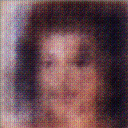
\includegraphics[width=150px]{500_fake_images/samples_5_100.png}%
\caption{A Man In A Black Shirt And A Tie}%
\end{figure}

%
\end{document}